


\documentclass[runningheads,a4paper]{llncs}
\usepackage{amssymb}
\setcounter{tocdepth}{3}
\usepackage{multirow}
\usepackage{graphicx}
\usepackage{epsfig}
\usepackage{xcolor}
\usepackage{times}
\usepackage{graphicx}
\usepackage{mwe}    \usepackage{subfig}
\usepackage[numbers,sort]{natbib}
\renewcommand{\bibname}{References}
\renewcommand{\bibsection}{\subsection*{References}~\\[-8ex]}
\usepackage{booktabs}
\usepackage[hyphens]{url}
\renewcommand{\ttdefault}{cmtt}

\urldef{\mailsa}\path|{,|
\urldef{\mailsb}\path|,|
\urldef{\mailsc}\path| }@unimelb.edu.au|    
\newcommand{\keywords}[1]{\par\addvspace\baselineskip
\noindent\keywordname\enspace\ignorespaces#1}


\newcommand{\D}{\hphantom{0}}
\newcommand{\C}{\hphantom{0,}}
\newcommand{\var}[1]{\mbox{\emph{#1}}}

\newcommand{\todo}[1]{[[{\emph{#1}}]]}

\newcommand{\alicia}[1]{\textcolor{magenta}{Alicia says: #1}}
\newcommand{\andrew}[1]{\textcolor{blue}{Andrew says: #1}}
\newcommand{\alistair}[1]{\textcolor{orange}{Alistair says: #1}}

\newcommand{\myparagraph}[1]{\vspace*{-0.7ex}\paragraph*{\normalsize\bf{#1}}}

\newcommand{\treceval}{{\tt\small{trec\_eval}}}
 
\begin{document}

\mainmatter  
\title{How Precise Does Document Scoring Need To Be?}

\titlerunning{How Precise Does Document Scoring Need To Be?}

\author{Ziying Yang \and Alistair Moffat \and Andrew Turpin}\authorrunning{Yang, Moffat, Turpin}

\institute{
Department of Computing and Information Systems,\\
The University of Melbourne, Australia\\
}


\toctitle{How Precise Does Document Scoring Need To Be?}
\tocauthor{Ziying Yang, Alistair Moffat, and Andrew Turpin}
\maketitle

\begin{abstract}
We explore the implications of tied scores arising in the document
similarity scoring regimes that are used when queries are processed
in a retrieval engine.
Our investigation has two parts: first, we evaluate past TREC runs to
determine the prevalence and impact of tied scores, to understand the
alternative treatments that might be used to handle them; and second,
we explore the implications of what might be thought of as
``deliberate'' tied scores, in order to allow for faster search.
In the first part of our investigation we show that while tied scores
had the potential to be disruptive to TREC evaluations, in
practice their effect was relatively minor.
The second part of our exploration helps understand why that was so,
and shows that quite marked levels of score rounding can be
tolerated, without greatly affecting the ability to compare between
systems.
The latter finding offers the potential for approximate scoring
regimes that provide faster query processing with little or no loss
of effectiveness.
\end{abstract}
 \section{Introduction}
\label{sec-intro}

Batch evaluation techniques are widely used in information retrieval
system measurement.
Each system that is to be compared generates a ranking, or
{\emph{run}}, for each of a set of topics, with documents included in
the run and also ordered within the run on the basis of some computed
textual {\emph{similarity score}} relative to the given query.
Possible similarity computations include the Okapi BM25 mechanism of
{\citet{rwjhg94trec}} and the language modeling techniques of
{\citet{pc98sigir}}.
Static score components such as Pagerank or other assessments of
document quality can also be included.
Those runs are then mapped to numeric {\emph{effectiveness values}}
using a set of relevance judgments and an {\emph{effectiveness
metric}}, which generates a single number as an assessment of the
quality, or utility, of that run in the eyes of the user that is
presumed to have inspected it.
Finally, the effectiveness values are aggregated in some way across
topics to get an overall performance measure which is often used,
with a suitable statistical test, as a basis for answering the
question ``is System A demonstrably better than System~B?''.

In this work we consider the consequences of allowing {\emph{tied
similarity scores}} (or just {\emph{ties}}) in the ranking.
The obvious issue is that ties admit a level of ambiguity in the
effectiveness metric values, and hence (potentially) in the outcome
of a system versus system comparison, since a group of documents that
all share the same computed similarity score could be presented to
the user in any permutation that is consistent with the scores being
non-increasing.
Our first goal is thus to quantify the extent to which past Text
Retrieval Conference (TREC) evaluation exercises have been affected
by tied similarity scores, and determine whether the presence of
ties may have caused ambiguity to flow through into system
scores.
In this part of the project we make use of a range of tie-breaking
regimes, including the rules embedded in the well-known
{\treceval} program, and conclude that while ties have had the
potential to be significantly disruptive, in practice they did not
influence the outcomes of the measurements that were undertaken.

A second related goal is to ask whether the deliberate introduction
of ties might be useful in some way.
For example, a range of approaches in which similarity scoring might
be approximated or otherwise quantized have been suggested over the
years including, for example
the quantized document weights of {\citet{mzs94ipm}}, or
the impact-ordered indexes of {\citet{am06sigir}}.
If we allow that the retrieval system might gain tangible efficiency
benefits from assigning scores with low precision to
documents,
then we may end up with large
numbers of ties in the runs that the system generates,
and being able to estimate the extent to which ties can
be tolerated before there is risk of degraded system retrieval
effectiveness is a key component of the approximation.
In experiments using submitted TREC runs, we show that quite marked
levels of approximation can be tolerated before system scores change
significantly, and hence that relatively low-precision scoring can be
employed if it boosts efficiency.

 \section{Ties, and Methods for Dealing With Them}
\label{sec-ties}

\myparagraph{Terminology}

We suppose that the similarity scores generated for a query partition
the document ranking -- the {\emph{run}} -- into {\emph{groups}}
within which the documents have the same score.
Let $b_g$ be the rank in the run at which the $g$\,th equi-score
group commences, with, by definition, $b_1=1$; and let $e_g$ be the
rank of the last document in that group, with $b_{g+1}=e_g+1$.
That is, the $g$\,th group of tied documents spans the items
$[b_g\ldots e_g]$, and contains $s_g=b_{g+1}-b_g$ documents.
We further define $G_g$ to be the multiset of gain values associated
with the documents in the $g$\,th group,
	$G_g =\{r_k\mid b_g \le k \le e_g\}$, 
with $r_k\in\{0,1\}$ the gain associated with the document at rank $k$;
and define $t_g$
to be the total gain associated with the $g$\,th group,
	$t_g = \sum \{r_k\mid b_g \le k \le e_g\}$.
For example, consider the ten-item ranking shown in
Figure~\ref{fig-example}, with each document given a single letter
label for convenience, and with five different computed similarity
scores.
The second row shows a presumed relevance value for each
corresponding document (``$0$'' and ``1''); and the third row lists
the similarity scores that are presumed to have led to that ranking.

If the scores are ignored and only the list of relevance values is
employed, computation of (for example) the metric precision at depth
$k=5$ (P@$5$) yields a score of $2/5=0.4$, because there are two
``$1$''s among the first five gain values.
Similarly, the ranking shown has a reciprocal rank (RR) score of
$1/3=0.333$, since the first relevant document appears at rank $k=3$.
Other metrics such as average precision (AP), rank-biased precision
(RBP) {\citep{mz08acmtois}}, and normalized discounted cumulative
gain (NDCG) {\citep{jk02acmtois}}, can also be computed, based solely
on that third ``gain'' row, without consideration of the document
labels in the first row, or their scores in the second row.

\begin{figure}[t]
\centering
\newcommand{\tabent}[1]{\makebox[18mm][l]{#1}}
\begin{tabular}{l|@{\hspace{1.0em}} *{10}{l@{\hspace{1.8em}}}}
\tabent{rank, $k$}
	& 1
	    & 2
	    	& 3
		    & 4
		    	& 5
		            & 6
			    	& 7
			    	    & 8
				        & 9
					    & 10
\\
\hline
\tabent{document, $d_k$}
	& D
	    & H
	        & A
		    & C
		        & M
			    & S
			        & W
				    & B
				        & E
					    & J
\\
\tabent{gain, $r_k$}
	& 0
	    & 0
	        & 1
		    & 1
		        & 0
			    & 1
			        & 1
				    & 0
				        & 0
					    & 1
\\
\tabent{score}
	& 9.8
	    & 9.3
	        & 9.3
		    & 9.3
		        & 8.4
			    & 8.4
			        & 8.2
				    & 8.0
				        & 8.0
					    & 8.0
\\
\tabent{groups}
	& \multicolumn{1}{@{}l}{$b_1{=}1$}
	    & \multicolumn{1}{@{}l}{$b_2{=}2$}
	        &
		    &
		        & \multicolumn{1}{@{}l}{$b_3{=}5$}
			    &
			        & \multicolumn{1}{@{}l}{$b_4{=}7$}
				    & \multicolumn{1}{@{}l}{$b_5{=}8$}
				        &
				            &
\\
\end{tabular}
 \caption{Example run showing five equi-score groups.
\label{fig-example}}
\end{figure}

When scores are included, the situation changes.
Now documents M and S can be seen to have the same similarity score,
and are part of a tied group.
That means that P@$5$ might be either $2/5$ or $3/5$, depending on
the tie-breaking rule employed to order them.
Similarly, RR might be $1/2$ or $1/3$, because of the tie involving
documents H and A and C (but note that there is no
possible arrangement in which RR can be $1/4$).

\myparagraph{Run Order}

A range of mechanisms have evolved to deal with tied scores.
The first and most obvious option is to do as has already been
suggested in connection with the example shown in
Figure~\ref{fig-example}, and that is to ignore the document scores
and process the run in the order in which the documents are presented
-- in effect, pushing the responsibility for tie-breaking back to the
retrieval system, whether or not it accepts it.
This approach presumes that the system has employed more information
than is captured in the final score, perhaps via further precision in
the internal computation above and beyond what is passed to the
evaluation regime, or perhaps via a secondary-key ordering process
that is not part of the scores at all.
However the system's ordering arises, respecting the sequential
presentation of documents is a plausible default way of handling tied
scores.

\myparagraph{External Tie-Break Rule}

A second option is to make use of some external fixed ordering
criterion and use it to reorder the documents within each tied group,
thereby obtaining a canonical representation for the run.
For example, the documents in each group might be sorted according to
their document identifier, or according to their length, or according
to their URL or filename.
As one specific example of this type of approach, the widely-used
{\treceval} program (see
{\small\url{http://trec.nist.gov/trec_eval/}}) sorts tied groups into
decreasing order of document identifier before performing its various
effectiveness metric computations.

\myparagraph{Optimistic and Pessimistic Limits}

A third way of handling runs with ties is to compute the best and
worst scores that might arise, and then present a score range rather
than a score value.
The advantage of this approach is that it makes clear when scores
contain potential ambiguity, in a way that mirrors the residuals of
{\citet{mz08acmtois}}, which provide guidance as to the metric weight
assigned to unjudged documents.
To compute an optimistic upper score bound, the $t_g$ relevant
documents within the $g$\,th group are assumed to appear in the
first rank positions, that is, $[b_g\ldots b_g+t_g-1]$, and the
metric score then computed in the usual way.
Similarly, to get a pessimistic lower score bound, the $t_g$ relevant
documents in the group are assumed to appear as a block as deep in
the run as is possible, at ranks $[e_g-t_g+1\ldots e_g]$.
In the example shown in Figure~\ref{fig-example}, the ordering ``H
then A then C'' (and similarly in the other groups) is used to derive
a lower bound on the score, and the ordering ``A then C then H'' (and
so on) is used to obtain an upper bound.
If a document is unjudged, then for many metrics (but notably, not
for AP or NDCG) it should be assumed to be non-relevant for the
purposes of establishing the lower bound, and assumed to be relevant
for the purposes of establishing the upper bound.

\myparagraph{Averaging Across Permutations}

While the worst-case bounds can be informative, they are also
somewhat pessimistic, and computing the average, or expected, value
of the metric across all possible permutations of documents within
each of the tied score groups provides a useful balance.
If every permutation of documents in each group is equally likely,
then computing the expectation is simply the process of computing the
metric for each permutation and taking their average.
For a small number of small groups, this $O(\prod_g (s_g!))$
brute-force approach is computationally feasible.
But if there are many blocks, or if there are any large blocks, it is
expensive.
Fortunately, the summation over all permutations telescopes for most
metrics, leading to a tractable computation.
{\citet{mn08ecir}} describe this process in detail, and present an
incremental formulation for average precision that computes the
expected score across all possible permutations of documents in each
group.
A similar computation can be used to compute an expected (across
permutations within groups) RR score.

For weighted-precision metrics such as RBP, a similar process can be
adopted.
The set of gain values associated with each group is summed and
averaged, and then that average gain applied at each rank position,
and weighted according to the decay function.
For the example shown in Figure~\ref{fig-example}, and an RBP
parameter $p=0.5$, the expected RBP0.5 score is computed as
\newcommand{\mysub}[2]{{#1}_{\mbox{\scriptsize{\,#2}}}}
\[
		0.5\times
				\frac{0}{1}
	+
	(0.25+0.125+0.0625)\times
				\frac{2}{3}
	+
	(0.0313+0.0156)\times
				\frac{1}{2}
	+
	\cdots
\]
We use these formulations for expected AP, expected RR (not to be
confused with the metric ERR), and expected RBP in the experiments
described in the next two sections.
 \section{Ties in TREC Experimentation}
\label{sec-trecimpact}

\myparagraph{TREC Resources}

In this section we examine the role that ties may have had on past
TREC evaluations.
The primary resource we make use of are the $103$ runs submitted as
part of the 1998 TREC7 Ad-Hoc experimentation round
{\citep{vh98trec}}, see {\small\url{trec.nist.gov}}, and
{\citet{harman05trecbook}} for a broad overview.
Each run is a list of (up to) $1{,}000$ responses from that system
for each of $50$ topics, with each row in the run file including
fields for {\emph{docnum}}, {\emph{rank}}, and {\emph{score}}.
There are thus three possible ways that each run could be
interpreted:
\begin{itemize}
\item
by the line number ordering implicit in the presentation of the run;
\item
by (increasing, or at least, non-decreasing) values in the
{\emph{rank}} field;
\item
by (decreasing, or at least, non-increasing) values in the
{\emph{score}} field.
\end{itemize}
Line numbers are unique within each system-topic combination, and do
not admit ties, but both ranks and scores might provide ties in runs.
To explore the prevalence of ties, the TREC7 Ad-Hoc runs were
analyzed.
Somewhat surprisingly, we discovered that there were $254$ instances
in the archived runs where scores were increasing rather than
non-increasing in terms of the line ordering, and that five systems
were affected by this inconsistency.
The primary reason appears to be incorrect sorting of scores when
exponential formatting is being used.
For example, in the run {\tt{bbn1}}, for topic $355$, the
second-to-last score in the run is {\tt{-1.37}}; and final score is
{\tt{-7.763e-05}}.
In fact, that last document's correct position is some $700$
locations higher, at rank $304$, the rank that row was labeled with.
When rank ordering was similarly checked the situation was even more
confused, and $7.3$\% of the documents in the archived runs
($358{,}631$ entries in total) were mis-ordered according to their
stated ranks.
That is, the supplied document ordering in the runs corresponds to
neither increasing rank nor to non-decreasing score.

\begin{table}[t!]
\centering
\begin{tabular}{l c ccc}
\toprule
	&& \multicolumn{3}{c}{Percentage affected}
\\
\cmidrule{3-5}
	&& systems
		& system-topics
			& documents
\\
\midrule
Tied scores
	&& 95.2
		& 91.0
			& 14.0
\\
Rank/score contradictions
	&& \D6.8
		& \D4.2
			& \D1.4
\\
\bottomrule
\end{tabular}
 \renewcommand{\tabcolsep}{0.5em}
\caption{Ties occurring in $103$ TREC7 Ad-Hoc runs after score-based
re-sorting: the percentage of systems, system/topic combinations, and
documents that include tied scores; and the corresponding percentages
of score-rank contradictions.
There are $103$ systems, $103\times50$ system-topic
combinations, and $4{,}900{,}042$ documents.
Note that not all runs contain $1{,}000$ documents.
\label{tbl-trec7-ties}}
\end{table}

To resolve this apparent mislabeling, we re-sorted all of the TREC7
submissions, taking care to treat the exponential formats correctly.
We used decreasing numeric score as the primary key, and then
increasing rank as a secondary key.
This is guaranteed to give rise to runs in which there are no
score-based out-of-order items.
We then counted the occurrences of score ties at the document, topic,
and system level; and the occurrence of rank contradictions, where a
``contradiction'' is a pair of adjacent documents that when sorted by
score have ranks that indicate the opposite ordering.
Table~\ref{tbl-trec7-ties} shows the results of this processing.
As can be seen, $14$\% of the documents in the runs have the same
score as their predecessor document in that run, a fact that provides
the motivation for our work here; and, of equal concern, a further
$1.4$\% of the documents cannot be placed in a manner that is
consistent with both their assigned score and their assigned rank,
with seven of the $103$ systems affected.
We can only assume that the cause of the latter issue was programming
errors at the time the runs were created by the corresponding
research groups.
There were no ties on rank in any of the TREC7 runs.

To ensure that the results in the remainder of the paper were not
affected by programming mistakes and other experimental
misunderstandings on the part of the 1998 TREC7 participants, we then
took the top $80$ systems, as ordered by average AP score over the
$50$ topics, discarding the other $23$ systems from further
evaluation.
Similar restrictions have also been employed by other authors.


\myparagraph{Ties in TREC7}

\begin{figure}[t!]
\centering
\includegraphics[width=1\textwidth]{figs/fig-trec7-ap-scores.pdf}
\caption{Imprecision in AP scores caused by ties in a set of $80$
TREC7 runs.
\label{fig-trec7-ap-scores}}
\end{figure}

The primary evaluation metric used in TREC7 was average precision, as
implemented in the program {\treceval} (version 9.0).
Working with the $80$ score/rank-sorted runs, we next sought to
examine the effect that the score-ties had on AP scores for systems.
Figure~\ref{fig-trec7-ap-scores} plots those systems.
The horizontal axis is the {\treceval} score for that system,
expressed as a mean AP value over the $50$ topics.
By inspecting the {\treceval} source code we were able to confirm
that it (a) ignored line ordering in the input runs; (b) used
exponential number formats correctly when performing its
sorting-by-score step; and (c) resolved score ties by reverse sorting
on document number, paying no attention to the supplied {\emph{rank}}
field.
The scale on the vertical axis in Figure~\ref{fig-trec7-ap-scores} is
the AP score range measured by taking the difference between the
pessimal and optimal topic scores, and then averaging across topics
to get a system range.
The higher up the axis a system is plotted, the greater the
uncertainty in its score.

Each system is plotted as a segment.
The right and left ends of the segment reflect the scores that would
be generated by the optimistic and pessimistic orderings for each of
the tied groups; the {\treceval} score is shown as a circle; and the
``average across permutations'' score as a triangle.
The color of each point reflects the number of document ties for that
system, in terms of Table~\ref{tbl-trec7-ties}.
The vertical axis is truncated at $10^{-6}$, and the points plotted
along that line have a score difference of $10^{-6}$ or below.
At the top of the graph, many tied scores lead to wide score ranges,
with the {\treceval} ordering being just one of them, usually not too
far from the average overall.
But for some systems the optimal-to-pessimal spread is wide, and as
can be seen in the overlapping vertical extents, ties may have
affected the relative ordering of the top few systems ($\mbox{AP}\ge
0.30$).
At the bottom of the graph, only a tiny minority of systems have no
tied scores at all; but for most evaluations the ties that do exist
do not result in any appreciable score range, with
optimal-to-pessimal ranges less than $10^{-4}$ when averaged across
topics.


\myparagraph{Ties in Other Years}

We carried out the same analysis on several other TREC rounds, and
found similar rates of tied scores in general
(Table~\ref{tbl-trec7-ties}), and instances of systems with wide
potential score ranges.
However we found no further years in which the ordering of the
top few systems might have been affected by the tie-breaking rule
employed.


 \section{Deliberate Score Grouping}
\label{sec-roundingoff}

We now consider whether the deliberate use of tied scores
has a discernible effect on retrieval effectiveness.

\myparagraph{Score Approximation}

Scoring documents using modern similarity computations involves
non-trivial amounts of arithmetic, especially if phrase components or
term proximity components are being used.
Regimes such as WAND {\citep{bchsz03cikm}} seek to minimize the
number of documents scored, while still giving rise to exactly the
same ranking for the top-$k$ documents, an approach that meets the
requirements for being {\emph{rank-safe to depth~$k$}}.
That is, the WAND process ensures that all of the documents in the
first $k$ places of the ranking are in their right positions, but
makes no guarantee for documents beyond depth $k$.
This is a relatively stringent requirement, and other
computation-pruning techniques might also be considered that provide
more flexible trade-offs.

In particular, we now consider the following weaker requirement: that
each document must be scored in a manner that guarantees that it is
in the correct {\emph{band}} of the ranking, where the bands are
defined geometrically based on a parameter $\rho>1$.
More precisely, let $b_1=1$, and thereafter let
$b_{g+1}=\lceil{\rho\cdot b_g}\rceil$.
The $g$\,th band, for $g\ge1$, spans the ranks from $b_g$ to
$e_g=b_{g+1}-1$ inclusive.
For example, if $\rho=2$, then the bands are $[1\ldots1]$,
$[2\ldots3]$, $[4\ldots7]$, and so on; and if (say) $\rho=1.62$ (the
golden ratio) the bands are $[1\ldots1]$, $[2\ldots3]$, $[4\ldots6]$,
$[7\ldots11]$, and so on, with widths given by the Fibonacci
sequence.
The smaller the value of $\rho$, the smaller the band is that spans
any given position in the ranking, and the nearer the approximate
ranking is to the ``true'' and exact ranking.
In the limit, as $\rho$ approaches $1$, the retrieval system is
obliged to place each document at its final ``correct'' position; that is,
$\rho=1$ corresponds to a ``full'' computation in which all document
relationships are finalized.
But when $\rho>1$, we allow the retrieval system to economize on its
computational costs and return groups of documents $[b_g\ldots e_g]$,
with equal scores assumed within each band.

\myparagraph{Worst-Case Bounds}

It is straightforward to show that when $\rho>1$ the first group
containing more than one document starts at rank
$v=b_v=1+\lfloor{1/(\rho-1)}\rfloor$.
That fact implies that the approximate scoring mechanism is rank-safe
to depth $v-1$, and more generally, allows bounds on the imprecision
in scores to be computed.
For example, consider the metric reciprocal rank (RR).
With the $v$\,th group the first one with multiple documents in it,
the loss of score that can arise when permutation-based averaging is
applied is given by
\[
	\Delta\mbox{RR} = \frac{1}{b_v} -
		\frac{1}{e_v-b_v+1}\sum_{k=b_v}^{e_v} \frac{1}{k} \,,
\]
where the bound arises because the worst situation is when the
original run has its first relevant document at rank $b_v$, and no
other document in that group is relevant.
Table~\ref{tbl-bounds} gives some $\Delta$RR values; when $\rho\le2$,
all are less than $0.1$.


\begin{table}[t]
\centering
\renewcommand{\tabcolsep}{0.5em}
\newcommand{\tabent}[1]{\makebox[15mm][c]{#1}}
\begin{tabular}{l c ccc}
\toprule
\multirow{2}{*}{$\rho$}
	&& \multicolumn{3}{c}{Metric}
\\
\cmidrule{3-5}
	&& \tabent{RR}
		& \tabent{RBP0.5}
			& \tabent{RBP0.85}
\\
\midrule
1.1
	&& 0.0038
		& 0.0002
			& 0.0087
\\
1.2
	&& 0.0119
		& 0.0052
			& 0.0231
\\
1.4
	&& 0.0417
		& 0.0429
			& 0.0482
\\
1.7
	&& 0.0833
		& 0.0945
			& 0.0777
\\
2.0
	&& 0.0833
		& 0.1016
			& 0.0971
\\
\bottomrule
\end{tabular}
 \caption{Worst-case metric score differences associated with geometric
grouping of documents in runs, controlled by parameter $\rho$.
It is not possible to derive equivalent bounds for AP.
\label{tbl-bounds}}
\end{table}

It is also possible to compute worst-case differences for rank-biased
precision (RBP, see {\citet{mz08acmtois}}).
In the case of RBP, the maximum difference score difference arises
when the run has a sequence of relevant documents at the start of
each of its groups, followed by non-relevant documents for the rest
of each group.
The exact number $1\le t_g \le (e_g+b_g)/2$ of relevant documents
required in the initial run for the $g$\,th group varies according to
both $p$ (the RBP parameter) and $\rho$, and is chosen independently
in each group to maximize the difference
\[
		\left(
	\sum_{k=b_g}^{b_g+t_g-1} (1-p)p^{k-1}
	\right)
	-
	\left(
	\frac{t_g\cdot w_g}{e_g-b_g+1}
	\right) \, ,
\]
where $w_g=\sum_{k=b_g}^{e_g} (1-p)p^{k-1}$ is the sum of the RBP
weights associated with that $g$\,th group.
The overall bound on the difference, $\Delta$RBP, is the sum of the
group maximum differences.
Table~\ref{tbl-bounds} includes $\Delta$RBP differences for two
values of the RBP parameter~$p$.
Recall-based metrics such as average precision (AP) cannot be
analyzed as readily, because assuming additional documents to be
relevant might decrease rather than increase the score.
Experimental results showing that practice that AP has less
divergence of scores than does RBP are presented in the next
subsection.


\myparagraph{Effectiveness Score Differences in Practice}

Given these worst-case bounds, the next question we ask is this: to
what extent does an allowance for rank-based score imprecision affect
effectiveness scores in practice?
To respond to this question, we again make use of the 1998 TREC7
resources, taking the same system runs as were already examined in
Section~\ref{sec-trecimpact}, and for each run, mapping it to a set
of equivalent banded runs based on a set of $\rho$ values, with the
documents ranked in band $g$ in each of those runs assigned a
synthetic score of $1/g$.
The original system scores that were part of the TREC7 data were
ignored as the grouping operation was being carried out, and original
file order was used as the reference point for each run.
As already detailed in Section~\ref{sec-trecimpact}, $23$ low-scoring
systems were removed as part of the experimental methodology.

\begin{figure}[t!]
\centering
\subfloat[RR\label{fig-score-variation-rr}]{\includegraphics[width=0.49\textwidth]{figs/fig-score-variation-rr.pdf}
}
\subfloat[RBP0.5\label{fig-score-variation-rbp50}]{\includegraphics[width=0.49\textwidth]{figs/fig-score-variation-rbp50.pdf}
}
\\
\subfloat[RBP0.85\label{fig-score-variation-rbp85}]{\includegraphics[width=0.49\textwidth]{figs/fig-score-variation-rbp85.pdf}
}
\subfloat[AP\label{fig-score-variation-ap}]{\includegraphics[width=0.49\textwidth]{figs/fig-score-variation-ap.pdf}
}
\caption{Variation in metric effectiveness score across a set of $80$
runs and $50$ topics (that is, $50 \times 80$ points are plotted in
each column), as a function of $\rho$, for four different retrieval
effectiveness metrics.
The whiskers indicate the last outlier still within $1.5$ times of
the inter-quartile range from the corresponding quartile (the limits
of the boxes).
\label{fig-score-variation}}
\end{figure}

Figure~\ref{fig-score-variation} shows the results of this
experimentation, plotted as a sequence of box-whisker elements using
four different effectiveness metrics and a single representative
value of $\rho=1.4$.
In all cases the score difference calculated is the
across-permutations computation that was illustrated in
Section~\ref{sec-ties} when applied to the deliberately-tied
rankings, subtracted from the score the same metric achieved on the
original submitted ranking for that same topic.
We followed standard protocols and assumed that unjudged documents
were not relevant for the purposes of scoring the runs.

Figure~\ref{fig-score-variation} shows that the average score
variation arising from the banding process is small, and that there
are nearly as many system-topic combinations that gain from the
approximation process as there are that lose from it.
Most RR values are unaffected (both quartiles are zero, for all of
the $\rho$ values tested), and the two deep metrics (RBP0.85 and
AP) also have small inter-quartile ranges on the computed score
differences.
The average original metric scores across all system-topic
combinations for RR, RBP0.5, RBP0.85, and AP are, respectively,
$0.6939$, $0.5556$, $0.4677$, and $0.2311$; and hence the
smaller AP score differences are in part a matter of relative scale.
The shallow metric RBP0.5 suffers the most from the score grouping
process; even so, it is only when $\rho>1.5$, the first value for
which ranks $2$ and $3$ are placed in the same group, that the
differences are large.
When  $\rho\le2$ the first group always contains a
single document.

\begin{table}[t!]
\centering
\renewcommand{\tabcolsep}{0.5em}
\newcommand{\tabent}[1]{\makebox[9mm][c]{#1}}
\begin{tabular}{l c cccc c cccc}
\toprule
\multirow{2}{*}{$\rho$}
	&& \multicolumn{4}{c}{Relative to $99$\% of original score}
		&& \multicolumn{4}{c}{Relative to $97$\% of original score}
\\
\cmidrule{3-6}\cmidrule{8-11}
	&& \tabent{RR}
		& \tabent{RBP0.5}
			& \tabent{RBP0.85}
				& \tabent{AP}
					&& \tabent{RR}
						& \tabent{RBP0.5}
							& \tabent{RBP0.85}
								& \tabent{AP}
\\
\midrule
1.1
	&& 80
		& 80
			& 80
				& 80
					&& 80
						& 80
							& 80
								& 80
\\
1.2
	&& 80
		& 80
			& 80
				& 80
					&& 80
						& 80
							& 80
								& 80
\\
1.4
	&& 77
		& 44
			& 65
				& 44
					&& 80
						& 80
							& 80
								& 80
\\
1.7
	&& 37
		& 11
			& 14
				&\D0
					&& 80
						& 67
							& 80
								& 77
\\
2.0
	&& 38
		& 10
			&\D3
				&\D0
					&& 80
						& 61
							& 71
								& 20
\\
\bottomrule
\end{tabular}
 \caption{Number of systems (maximum $80$) for which a $t$-test across
$50$ topics yields confidence at the $p\le0.05$ level that the
grouped runs yield a metric score greater than or equal to $99$\%
(left) and $97$\% (right) of the original run score.
\label{tbl-frac-significant}}
\end{table}


Table~\ref{tbl-frac-significant} explores whether the small score
differences identified in Figure~\ref{fig-score-variation} can be
regarded as being significant.
To generate the table, each of the $80$ systems was scored for the
$50$ topics using the original runs, and then re-scored using the
grouped runs.
The set of original topic scores was then multiplied by $0.99$, and
compared to the grouped scores, using a one-tail paired $t$-test.
If a $p$ value less than or equal to $0.05$ was generated by that
test, that system was counted as being one for which the grouping
process degraded the system score by $1$\% or less.
The closer the count of such systems is to $80$, the greater the
confidence we can have that the grouping process will not give
notably inferior system scores overall, where ``notably inferior'' is
defined (at first) as being a $1$\% degradation in measured score.
Those values are shown in the left half of
Table~\ref{tbl-frac-significant}, and the corresponding counts when
``notably inferior'' is defined as being a $3$\% degradation are
shown in the right half.
The relationship between $\rho$ and score fidelity is
reflected by the decreasing numbers down each column of the table,
and as $\rho$ increases, the possible implications of changes in
score also increase.
When the ``tolerable degradation limit'' was further reduced to
$95$\%, all $16$ entries for metric and $\rho$ were $80$.

\myparagraph{System Comparison Sensitivity}

Effectiveness measurements are also used to compare systems in a
pairwise manner.
In a final experiment, we explore the implications that score
rounding has on the ability of metrics to differentiate between
systems.
The normal approach to comparing systems is to take their computed
scores across a set of topics, and perform a paired $t$-test to
explore the null hypothesis that the two systems are in fact the
same.
The process of carrying out the $t$-test generates a $p$ value; the
smaller the $p$ value, the smaller the chance that the two systems
being compared are giving the same performance on the data used.
To establish significance, a threshold value $\alpha$ is employed,
often $\alpha=0.05$, with $p\le\alpha$ being regarded as a
significant outcome.

\begin{figure}[t!]
\centering
\includegraphics[width=0.95\textwidth,page=5]{figs/p_value_scatter_sys_pairs.pdf}
\caption{Correlation of $p$ values for all pairs of systems
($80\times79/2=3{,}160$ points per pane), with the $p$ value from a
paired $t$-test using the original system scores across $50$ topics
plotted on the horizontal axis, and the $p$ value for the
corresponding system pair with grouped runs ($\rho=1.4$) on the
vertical axis.
The dotted lines at are $p=0.05$, with the grid showing the
percentage of data points in each quadrant.
\label{fig-pair-variation}}
\end{figure}

To measure the effect that score rounding has on system comparisons,
we took the $50$ topics of the TREC7 collection and the $80$ runs
associated with it that we have been using, and computed, for each of
eleven different values of $\rho$, the set of $p$ values generated
for the $80\times79/2$ distinct system pairs.
In all cases when $\rho>1$, the averaging processes described in
Section~\ref{sec-ties} were used; when $\rho=1$, each run was
processed in sorted-by-score order, and then the scores were
discarded.

Figure~\ref{fig-pair-variation} shows that score grouping has almost
no effect at all on the ability to distinguish between systems using
a statistical test (the {\emph{discrimination ratio}} of the metric,
see {\citet{sakai07sigir}}), across the four metrics used in our
experiments.
For example, the plot in the lower-right for AP shows when $\rho=1.0$
that $62.2$\% of the system pairs yield ``significant at $p=0.05$''
comparison outcomes; at $\rho=1.4$, that fraction is $62.1\%$, with
only $0.1$\% of false positives, and $0.2$\% false negatives.
The situation is similar for the other metrics, with the
discrimination ratios (down to $45$\% for RR) determined primrily by
the effective evaluation depth, and only a small fraction of false
positives and negatives.
 \section{Conclusion and Future Work}
\label{sec-conclusion}

We have explored the impact of score ties on the evaluation of
retrieval system effectiveness, as measured using binary relevance
judgments and three established effectiveness metrics.
Ties have the potential to affect system comparisons, and using TREC
data, we showed that a small number of systems did indeed generate
runs with very ambiguous score outcomes, but that -- fortunately --
the overall conclusions from those rounds of experimentation were
unlikely to have been compromised.
We further demonstrated that allowing a controlled grouping of scores
in runs -- in a sense, permitting the deliberate introduction of ties
-- resulted in only small changes in the ability to compare systems.
This approach represents a novel direction in which retrieval
efficiency improvements might be achieved.
We have not yet addressed the question of how those efficiency gains
might be achieved, and a clear direction for future work is to
reexamine the computation embedded in standard similarity scoring
regimes and existing dynamic pruning heuristics, to identify and
measure ways in which processing economies might accrue through the
use of inexact scoring.

Another area for future work is in the space of test collection
construction.
Previous investigations
{\citep{voorhees00ipm,bcstvy08sigir,sst11sigir}} have explored the
reliability and quality of the collected judgments; it may be that
the pooled documents can be stratified according to the groups they
appear in, and less emphasis placed on judgment quality for deeper
pools, relying instead on averaging effects to preserve overall
evaluation quality.

 


\begin{small}
\renewcommand{\bibsep}{2.5pt}
\bibliographystyle{splncsnat}
\begin{thebibliography}{14}
\providecommand{\natexlab}[1]{#1}
\providecommand{\url}[1]{\texttt{#1}}
\providecommand{\urlprefix}{}

\bibitem[{Anh and Moffat(2006)}]{am06sigir}
Anh, V.N., Moffat, A.: Pruned query evaluation using pre-computed impacts.
\newblock In: Proc. SIGIR. pp. 372--379 (2006)

\bibitem[{Bailey et~al.(2008)Bailey, Craswell, Soboroff, Thomas, {de V}ries,
  and Yilmaz}]{bcstvy08sigir}
Bailey, P., Craswell, N., Soboroff, I., Thomas, P., {de V}ries, A.P., Yilmaz,
  E.: Relevance assessment: {A}re judges exchangeable and does it matter.
\newblock In: Proc. SIGIR. pp. 667--674 (2008)

\bibitem[{Broder et~al.(2003)Broder, Carmel, Herscovici, Soffer, and
  Zien}]{bchsz03cikm}
Broder, A.Z., Carmel, D., Herscovici, M., Soffer, A., Zien, J.: Efficient query
  evaluation using a two-level retrieval process.
\newblock In: Proc. CIKM. pp. 426--434 (2003)

\bibitem[{Harman(2005)}]{harman05trecbook}
Harman, D.K.: The {TREC} test collections.
\newblock In: Voorhees, E.M., Harman, D.K. (eds.) {TREC}: Experiment and
  Evaluation in Information Retrieval, chap.~2, pp. 21--52. MIT Press (2005)

\bibitem[{J\"arvelin and Kek\"al\"ainen(2002)}]{jk02acmtois}
J\"arvelin, K., Kek\"al\"ainen, J.: Cumulated gain-based evaluation of {IR}
  techniques.
\newblock ACM Trans. Inf. Sys. 20(4), 422--446 (2002)

\bibitem[{Mc{S}herry and Najork(2008)}]{mn08ecir}
Mc{S}herry, F., Najork, M.: Computing information retrieval performance
  measures efficiently in the presence of tied scores.
\newblock In: Proc. ECIR. pp. 414--421 (2008)

\bibitem[{Moffat and Zobel(2008)}]{mz08acmtois}
Moffat, A., Zobel, J.: Rank-biased precision for measurement of retrieval
  effectiveness.
\newblock ACM Trans. Inf. Sys. 27(1), 2.1--2.27 (2008)

\bibitem[{Moffat et~al.(1994)Moffat, Zobel, and Sacks-{D}avis}]{mzs94ipm}
Moffat, A., Zobel, J., Sacks-{D}avis, R.: Memory efficient ranking.
\newblock Inf. Proc. \& Man. 30(6), 733--744 (1994)

\bibitem[{Ponte and Croft(1998)}]{pc98sigir}
Ponte, J.M., Croft, W.B.: A language modeling approach to information
  retrieval.
\newblock In: Proc. SIGIR. pp. 275--281 (1998)

\bibitem[{Robertson et~al.(1994)Robertson, Walker, Jones, Hancock-{B}eaulieu,
  and Gatford}]{rwjhg94trec}
Robertson, S.E., Walker, S., Jones, S., Hancock-{B}eaulieu, M., Gatford, M.:
  Okapi at {TREC}-3.
\newblock In: Proc. TREC. pp. 109--126 (1994)

\bibitem[{Sakai(2007)}]{sakai07sigir}
Sakai, T.: Alternatives to {BP}ref.
\newblock In: Proc. SIGIR. pp. 71--78 (2007)

\bibitem[{Scholer et~al.(2011)Scholer, Turpin, and Sanderson}]{sst11sigir}
Scholer, F., Turpin, A., Sanderson, M.: Quantifying test collection quality
  based on the consistency of relevance judgements.
\newblock In: Proc. SIGIR. pp. 1063--1072 (2011)

\bibitem[{Voorhees and Harman(1998)}]{vh98trec}
Voorhees, E.M., Harman, D.K.: Overview of the {S}eventh {T}ext {RE}trieval
  {C}onference ({TREC}-7).
\newblock In: Proc. TREC. pp. 1--23 (1998), nIST Special Publication 500-242

\bibitem[{Voorhees(2000)}]{voorhees00ipm}
Voorhees, E.M.: Variations in relevance judgements and the measurement of
  retrieval effectiveness.
\newblock Inf. Proc. \& Man. 36(5), 697--716 (2000)

\end{thebibliography}
 
\end{small}

\end{document}
